% GNUPLOT: LaTeX picture with Postscript
\begingroup
  \makeatletter
  \providecommand\color[2][]{%
    \GenericError{(gnuplot) \space\space\space\@spaces}{%
      Package color not loaded in conjunction with
      terminal option `colourtext'%
    }{See the gnuplot documentation for explanation.%
    }{Either use 'blacktext' in gnuplot or load the package
      color.sty in LaTeX.}%
    \renewcommand\color[2][]{}%
  }%
  \providecommand\includegraphics[2][]{%
    \GenericError{(gnuplot) \space\space\space\@spaces}{%
      Package graphicx or graphics not loaded%
    }{See the gnuplot documentation for explanation.%
    }{The gnuplot epslatex terminal needs graphicx.sty or graphics.sty.}%
    \renewcommand\includegraphics[2][]{}%
  }%
  \providecommand\rotatebox[2]{#2}%
  \@ifundefined{ifGPcolor}{%
    \newif\ifGPcolor
    \GPcolortrue
  }{}%
  \@ifundefined{ifGPblacktext}{%
    \newif\ifGPblacktext
    \GPblacktexttrue
  }{}%
  % define a \g@addto@macro without @ in the name:
  \let\gplgaddtomacro\g@addto@macro
  % define empty templates for all commands taking text:
  \gdef\gplbacktext{}%
  \gdef\gplfronttext{}%
  \makeatother
  \ifGPblacktext
    % no textcolor at all
    \def\colorrgb#1{}%
    \def\colorgray#1{}%
  \else
    % gray or color?
    \ifGPcolor
      \def\colorrgb#1{\color[rgb]{#1}}%
      \def\colorgray#1{\color[gray]{#1}}%
      \expandafter\def\csname LTw\endcsname{\color{white}}%
      \expandafter\def\csname LTb\endcsname{\color{black}}%
      \expandafter\def\csname LTa\endcsname{\color{black}}%
      \expandafter\def\csname LT0\endcsname{\color[rgb]{1,0,0}}%
      \expandafter\def\csname LT1\endcsname{\color[rgb]{0,1,0}}%
      \expandafter\def\csname LT2\endcsname{\color[rgb]{0,0,1}}%
      \expandafter\def\csname LT3\endcsname{\color[rgb]{1,0,1}}%
      \expandafter\def\csname LT4\endcsname{\color[rgb]{0,1,1}}%
      \expandafter\def\csname LT5\endcsname{\color[rgb]{1,1,0}}%
      \expandafter\def\csname LT6\endcsname{\color[rgb]{0,0,0}}%
      \expandafter\def\csname LT7\endcsname{\color[rgb]{1,0.3,0}}%
      \expandafter\def\csname LT8\endcsname{\color[rgb]{0.5,0.5,0.5}}%
    \else
      % gray
      \def\colorrgb#1{\color{black}}%
      \def\colorgray#1{\color[gray]{#1}}%
      \expandafter\def\csname LTw\endcsname{\color{white}}%
      \expandafter\def\csname LTb\endcsname{\color{black}}%
      \expandafter\def\csname LTa\endcsname{\color{black}}%
      \expandafter\def\csname LT0\endcsname{\color{black}}%
      \expandafter\def\csname LT1\endcsname{\color{black}}%
      \expandafter\def\csname LT2\endcsname{\color{black}}%
      \expandafter\def\csname LT3\endcsname{\color{black}}%
      \expandafter\def\csname LT4\endcsname{\color{black}}%
      \expandafter\def\csname LT5\endcsname{\color{black}}%
      \expandafter\def\csname LT6\endcsname{\color{black}}%
      \expandafter\def\csname LT7\endcsname{\color{black}}%
      \expandafter\def\csname LT8\endcsname{\color{black}}%
    \fi
  \fi
    \setlength{\unitlength}{0.0500bp}%
    \ifx\gptboxheight\undefined%
      \newlength{\gptboxheight}%
      \newlength{\gptboxwidth}%
      \newsavebox{\gptboxtext}%
    \fi%
    \setlength{\fboxrule}{0.5pt}%
    \setlength{\fboxsep}{1pt}%
    \definecolor{tbcol}{rgb}{1,1,1}%
\begin{picture}(3680.00,3680.00)%
    \gplgaddtomacro\gplbacktext{%
      \csname LTb\endcsname%%
      \put(714,959){\makebox(0,0)[r]{\strut{}$-150$}}%
      \csname LTb\endcsname%%
      \put(714,1314){\makebox(0,0)[r]{\strut{}$-100$}}%
      \csname LTb\endcsname%%
      \put(714,1668){\makebox(0,0)[r]{\strut{}$-50$}}%
      \csname LTb\endcsname%%
      \put(714,2023){\makebox(0,0)[r]{\strut{}$0$}}%
      \csname LTb\endcsname%%
      \put(714,2378){\makebox(0,0)[r]{\strut{}$50$}}%
      \csname LTb\endcsname%%
      \put(714,2732){\makebox(0,0)[r]{\strut{}$100$}}%
      \csname LTb\endcsname%%
      \put(714,3087){\makebox(0,0)[r]{\strut{}$150$}}%
      \csname LTb\endcsname%%
      \put(812,570){\makebox(0,0){\strut{}$-180$}}%
      \csname LTb\endcsname%%
      \put(1237,570){\makebox(0,0){\strut{}$-120$}}%
      \csname LTb\endcsname%%
      \put(1663,570){\makebox(0,0){\strut{}$-60$}}%
      \csname LTb\endcsname%%
      \put(2089,570){\makebox(0,0){\strut{}$0$}}%
      \csname LTb\endcsname%%
      \put(2514,570){\makebox(0,0){\strut{}$60$}}%
      \csname LTb\endcsname%%
      \put(2940,570){\makebox(0,0){\strut{}$120$}}%
      \csname LTb\endcsname%%
      \put(3366,570){\makebox(0,0){\strut{}$180$}}%
    }%
    \gplgaddtomacro\gplfronttext{%
      \csname LTb\endcsname%%
      \put(357,2023){\rotatebox{-270.00}{\makebox(0,0){\normalsize $\Psi$}}}%
      \csname LTb\endcsname%%
      \put(2089,306){\makebox(0,0){\normalsize $\Phi$}}%
      \csname LTb\endcsname%%
      \put(1770,2270){\rotatebox{-65.00}{\makebox(0,0){\strut{}\textcolor{black}{\footnotesize 500}}}}%
      \csname LTb\endcsname%%
      \put(2378,2036){\rotatebox{127.00}{\makebox(0,0){\strut{}\textcolor{black}{\footnotesize 400}}}}%
      \csname LTb\endcsname%%
      \put(1783,1948){\rotatebox{-45.00}{\makebox(0,0){\strut{}\textcolor{black}{\footnotesize 400}}}}%
      \csname LTb\endcsname%%
      \put(2029,2484){\rotatebox{152.00}{\makebox(0,0){\strut{}\textcolor{black}{\footnotesize 300}}}}%
      \csname LTb\endcsname%%
      \put(1885,1759){\rotatebox{-38.00}{\makebox(0,0){\strut{}\textcolor{black}{\footnotesize 300}}}}%
      \csname LTb\endcsname%%
      \put(2670,1883){\rotatebox{110.00}{\makebox(0,0){\strut{}\textcolor{black}{\footnotesize 200}}}}%
      \csname LTb\endcsname%%
      \put(1477,2794){\rotatebox{-167.00}{\makebox(0,0){\strut{}\textcolor{black}{\footnotesize 200}}}}%
      \csname LTb\endcsname%%
      \put(2014,1527){\rotatebox{-32.00}{\makebox(0,0){\strut{}\textcolor{black}{\footnotesize 200}}}}%
      \csname LTb\endcsname%%
      \put(1196,2849){\rotatebox{33.00}{\makebox(0,0){\strut{}\textcolor{black}{\footnotesize 100}}}}%
      \csname LTb\endcsname%%
      \put(2481,2849){\rotatebox{51.00}{\makebox(0,0){\strut{}\textcolor{black}{\footnotesize 100}}}}%
      \csname LTb\endcsname%%
      \put(2699,2098){\rotatebox{-73.00}{\makebox(0,0){\strut{}\textcolor{black}{\footnotesize 100}}}}%
      \csname LTb\endcsname%%
      \put(1241,2426){\rotatebox{-30.00}{\makebox(0,0){\strut{}\textcolor{black}{\footnotesize 100}}}}%
      \csname LTb\endcsname%%
      \put(1284,1230){\rotatebox{-38.00}{\makebox(0,0){\strut{}\textcolor{black}{\footnotesize 100}}}}%
      \csname LTb\endcsname%%
      \put(2572,1068){\rotatebox{-46.00}{\makebox(0,0){\strut{}\textcolor{black}{\footnotesize 100}}}}%
      \csname LTb\endcsname%%
      \put(962,2336){\rotatebox{-155.00}{\makebox(0,0){\strut{}\textcolor{black}{\footnotesize 50}}}}%
      \csname LTb\endcsname%%
      \put(2958,2287){\rotatebox{-162.00}{\makebox(0,0){\strut{}\textcolor{black}{\footnotesize 50}}}}%
      \csname LTb\endcsname%%
      \put(1820,2873){\rotatebox{-46.00}{\makebox(0,0){\strut{}\textcolor{black}{\footnotesize 50}}}}%
      \csname LTb\endcsname%%
      \put(1885,1197){\rotatebox{49.00}{\makebox(0,0){\strut{}\textcolor{black}{\footnotesize 50}}}}%
    }%
    \gplbacktext
    \put(0,0){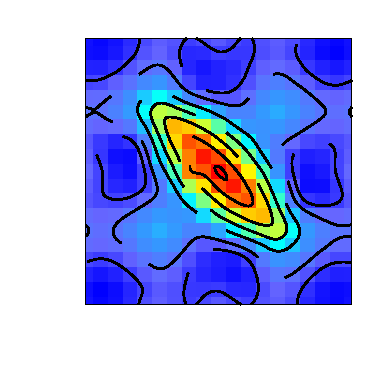
\includegraphics[width={184.00bp},height={184.00bp}]{Figs/Q0_E}}%
    \gplfronttext
  \end{picture}%
\endgroup
